%\documentclass[11pt,leqno]{book}
%\usepackage[spanish,activeacute]{babel}
%\usepackage[utf8]{inputenc}
%\usepackage{enumerate}
%
%\begin{document}

\chapter{Desarrollo informático}
\label{ch:informatica}

Para la realización de todos los experimentos en este capítulo (con excepción de los test estadísticos ANOVA y rangos múltiples, hechos en una versión de prueba de Statgraphics) se ha utilizado el software \texttt{R} junto con los paquetes \texttt{bmp} para leer imágenes en formato \textit{.bmp} y \texttt{gdpc} cuya versión en desarrollo puede encontrarse en el enlace en \cite{ezeq}. El resto de funciones utilizadas están en paquetes que se instalan en una instalación por defecto en \texttt{R}.

\section{Breve descripción del paquete utilizado}
y de las funciones que has hecho tú.

\section{Estudio de tiempos en función de los parámetros}


\section{Aplicación: Compresión de imágenes}

Vamos a ver como primera aplicación la compresión de imágenes tanto en escala de grises como a color. Se ha elegido esta aplicación porque las imágenes tienen la propiedad de que cada pixel se parece a los píxeles que tiene alrededor, de forma que si tomamos como cada serie temporal cada fila o columna de una imagen tenemos que las series se van a ir pareciendo entre sí, permitiendo obtener, en principio, pocas componentes principales con respecto al tamaño de la imagen y así tener un alto factor de compresión (que no es más que la reducción de dimensión de las series originales: las filas o columnas de la imagen).\\

Para aplicar el algoritmo GDPC (Generalized Dynamic Principal Components) a imágenes, se toman por tanto las columnas (o las filas) de una imagen como series temporales. El paquete \texttt{gdpc}, dada una matriz, toma como series temporales las columnas, por lo que a no ser que se especifique lo contrario, vamos a coger las columnas de la imagen como series temporales. De esta forma si la matriz tiene 500 filas por 300 columnas, tendríamos 300 series de 500 valores cada una. Para aplicar esto a imágenes a color, se toma cada capa R, G y B de la imagen a color como una matriz distinta y se sacan las componentes principales de cada matriz. Se han hecho experimentos con las siguientes tres imágenes, todas en formato \textit{.bmp} para que no hubiera una previa compresión de las mismas:
\begin{figure}[H]
 \centering
  \subfloat[Lena]{
   \label{f:lena}
    \includegraphics[width=0.32\textwidth]{../imagenes/LenaOriginal.pdf}}
  \subfloat[Pato]{
   \label{f:pato}
    \includegraphics[width=0.32\textwidth]{../imagenes/duckOriginal.pdf}}
  \subfloat[Tigre]{
   \label{f:tigre}
    \includegraphics[width=0.34\textwidth]{../imagenes/tigerOriginal.pdf}}
 \caption{Imágenes utilizadas}
 \label{f:imgs}
\end{figure}

Se han elegido las tres imágenes anteriores por las siguientes razones:
\begin{enumerate}
\item Hay una en escala de grises y dos a color, por lo que se ha podido experimentar con imágenes a color, que presentan 3 matrices distintas, una para cada canal de color.
\item Hay una imagen más sencilla, la del pato, y dos con más detalles, para comprobar cómo se comporta el algoritmo en cada caso.
\item Hay dos imágenes más grandes (Lena es de 512x512 y la del pato de 500x546) y una más pequeña, la del tigre, que tiene 320x240.
\end{enumerate}

Intuitivamente, en el primer punto deberíamos obtener que la imagen reconstruida en escala de grises tiene más calidad que las imágenes en color, puesto que al reconstruir tres capas en lugar de una hay más posibilidad de perder información general a la hora de ver la imagen. Del mismo modo, en el segundo punto se debería obtener que la imagen más sencilla tiene más calidad que las otras dos, ya que debe ser más fácil reconstruir una serie prácticamente constante.\\ %En cuanto al tercer punto, parecería lógico pensar que cuanto más pequeña sea la imagen más fácil será de reconstruir, ya que \\

En un primer experimento, se han sacado las componentes principales con \texttt{k\_max = 5} y \texttt{expl\_var = 0.95} en los tres casos y se han reconstruido las imágenes con las componentes y los coeficientes obtenidos. En el caso de las imágenes a color se han separado los canales de color, sacado las componentes principales para cada canal, se ha reconstruido cada canal con sus componentes y se han vuelto a juntar para guardar la imagen. En el caso de la imagen de Lena, se han obtenido 12 componentes principales dinámicas. Para el pato se han obtenido 6, 5 y 6 para las capas R, G y B, respectivamente, y para el tigre 10, 13 y 11. Los resultados obtenidos han sido los mostrados en las figuras \ref{f:imgsLena}, \ref{f:imgsPato} y \ref{f:imgsTigre}.\\

Es conveniente notar que para poder mostrar las imágenes ha habido que reescalar los valores obtenidos por la reconstrucción de las series a los intervalos $[0,255]$ en el caso de imágenes en blanco y negro y a $[0,1]$ en cada capa en el caso de imágenes a color. Esto ha sido así por las dos funciones de \texttt{R} que se han utilizado para dibujar las imágenes, \texttt{image()} para el primer caso y \texttt{rasterImage()} para el segundo. En \texttt{image()} se umbralizan directamente los valores que superan el 255 o que están por debajo del 0, sin embargo \texttt{rasterImage()} no, por lo que se ha procedido a hacerlo manualmente. En este caso no se podía umbralizar porque las capas originales estaban en el intervalo $[0,255]$ por lo que se ha utilizado el homeomorfismo de cambio del intervalo $[\text{min},\text{max}]$ al intervalo $[0,1]$:
\[	x^{'} = \frac{x - \text{min}}{\text{max}-\text{min}} 	\]
con $x \in [\text{min},\text{max}]$.

\begin{figure}[H]
 \centering
  \subfloat[Imagen original]{
   \label{f:lenaO}
    \includegraphics[width=0.5\textwidth]{../imagenes/LenaOriginal.pdf}}
  \subfloat[Imagen reconstruida]{
   \label{f:lenaR}
    \includegraphics[width=0.5\textwidth]{../imagenes/lena095.pdf}}
 \caption{Lena}
 \label{f:imgsLena}
\end{figure}

\begin{figure}
 \centering
  \subfloat[Imagen original]{
   \label{f:patoO}
    \includegraphics[width=0.5\textwidth]{../imagenes/duckOriginal.pdf}}
  \subfloat[Imagen reconstruida]{
   \label{f:patoR}
    \includegraphics[width=0.5\textwidth]{../imagenes/duck095.pdf}}
 \caption{Pato}
 \label{f:imgsPato}
\end{figure}

\begin{figure}
 \centering
  \subfloat[Imagen original]{
   \label{f:tigreO}
    \includegraphics[width=0.5\textwidth]{../imagenes/tigerOriginal.pdf}}
  \subfloat[Imagen reconstruida]{
   \label{f:tigreR}
    \includegraphics[width=0.5\textwidth]{../imagenes/tiger.pdf}}
 \caption{Tigre}
 \label{f:imgsTigre}
\end{figure}


Con estos experimentos podemos ver que en cuanto al segundo punto, las imágenes más simples no tienen por qué reconstruirse mejor, en contra de lo que se pensaba inicialmente, ya que la imagen más simple, que es la del pato, es la que peor se ve una vez se reconstruye. Esto es debido a que la mayor parte de las series en esa imagen (es decir, las columnas) son muy parecidas. De hecho, las componentes necesarias para explicar el 95\% de la varianza en esta imagen han sido menores que en las otras dos imágenes, concretamente la mitad de las componentes obtenidas con la imagen de Lena, que tiene casi la misma dimensión que la del pato, como se ha comentado antes. Esto implica que si los cambios en la imagen son pequeños (entendiendo como pequeños cambios suaves en el tono o color de la misma) normalmente se van a perder en la reconstrucción. Esto es lo que pasa por ejemplo con la parte del cuerpo del pato, donde está el detalle de las plumas. El cambio es demasiado suave entre todo el fondo amarillo y no es posible recogerlo en tan pocas componentes. Por esto, si los cambios son bruscos y las series difieren unas de otras harán falta más componentes para explicar el mismo porcentaje de varianza y por tanto el algoritmo tardará más pero también será mejor la reconstrucción. De esta forma, se explica que la imagen que peor se ve con respecto a la original sea la del pato, ya que tanto la de Lena como la del tigre tienen cambios más bruscos. De hecho, las partes de la imagen de Lena que son más uniformes en la imagen original se ven un poco peor en la imagen reconstruida.\\

Para ver esto más claro se ha cogido la imagen de Lena y se han hecho cambios en los niveles para pasar de una imagen prácticamente en negro a la imagen original. En este caso se ha hecho explicando el 90\% de varianza para reducir los tiempos de cómputo. Los resultados se pueden ver en las figuras \ref{f:imgsLenaN2}, \ref{f:imgsLenaN3}, \ref{f:imgsLenaN4}, \ref{f:imgsLenaN5} y \ref{f:imgsLenaN6}.\\

\begin{figure}
 \centering
  \subfloat[Imagen original]{
   \label{f:lenaN2O}
    \includegraphics[width=0.5\textwidth]{../imagenes/nivelesLena2.pdf}}
  \subfloat[Imagen reconstruida]{
   \label{f:lenaN2R}
    \includegraphics[width=0.5\textwidth]{../imagenes/nivelesLena2r.pdf}}
 \caption{Niveles de Lena}
 \label{f:imgsLenaN2}
\end{figure}

\begin{figure}
 \centering
  \subfloat[Imagen original]{
   \label{f:lenaN3O}
    \includegraphics[width=0.5\textwidth]{../imagenes/nivelesLena3.pdf}}
  \subfloat[Imagen reconstruida]{
   \label{f:lenaN3R}
    \includegraphics[width=0.5\textwidth]{../imagenes/nivelesLena3r.pdf}}
 \caption{Niveles de Lena}
 \label{f:imgsLenaN3}
\end{figure}

\begin{figure}
 \centering
  \subfloat[Imagen original]{
   \label{f:lenaN4O}
    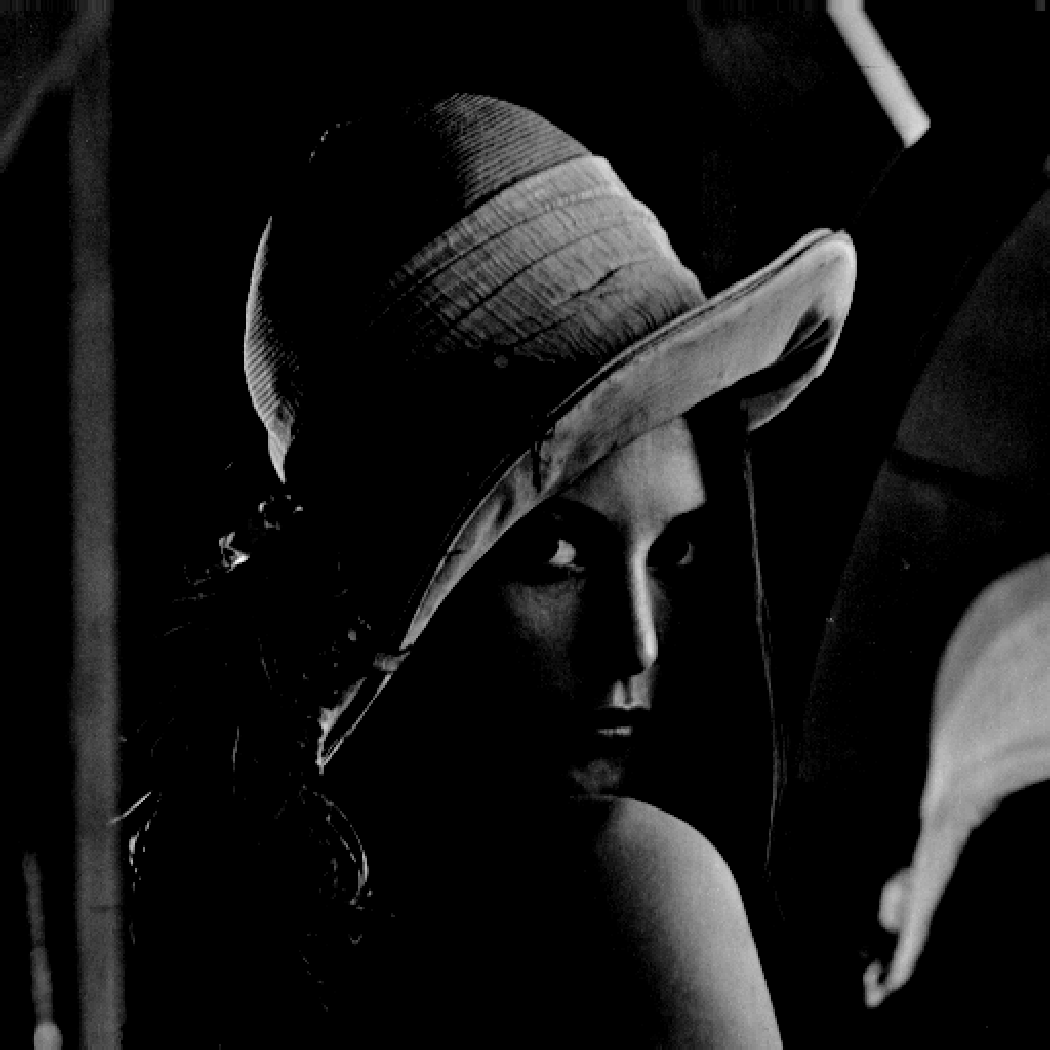
\includegraphics[width=0.5\textwidth]{../imagenes/nivelesLena4.pdf}}
  \subfloat[Imagen reconstruida]{
   \label{f:lenaN4R}
    \includegraphics[width=0.5\textwidth]{../imagenes/nivelesLena4r.pdf}}
 \caption{Niveles de Lena}
 \label{f:imgsLenaN4}
\end{figure}

\begin{figure}
 \centering
  \subfloat[Imagen original]{
   \label{f:lenaN5O}
    \includegraphics[width=0.5\textwidth]{../imagenes/nivelesLena5.pdf}}
  \subfloat[Imagen reconstruida]{
   \label{f:lenaN5R}
    \includegraphics[width=0.5\textwidth]{../imagenes/nivelesLena5r.pdf}}
 \caption{Niveles de Lena}
 \label{f:imgsLenaN5}
\end{figure}

\begin{figure}
 \centering
  \subfloat[Imagen original]{
   \label{f:lenaN6O}
    \includegraphics[width=0.5\textwidth]{../imagenes/nivelesLena6.pdf}}
  \subfloat[Imagen reconstruida]{
   \label{f:lenaN6R}
    \includegraphics[width=0.5\textwidth]{../imagenes/nivelesLena6r.pdf}}
 \caption{Niveles de Lena}
 \label{f:imgsLenaN6}
\end{figure}

En la figura \ref{f:imgsLenaN2} podemos ver que si la imagen está prácticamente en el mismo color y lo único que aparece en ella tiene mucho contraste, es decir, los cambios en la serie son bruscos, entonces la reconstrucción es bastante buena. Sin embargo en las figuras de la \ref{f:imgsLenaN3} a la \ref{f:imgsLenaN5} vamos viendo como según los cambios son menos bruscos y hay suficiente negro en la imagen, se van viendo peor las reconstrucciones para de nuevo, como podemos ver en la figura \ref{f:imgsLenaN6} y en la original, según van desapareciendo las partes constantes en negro y apareciendo los detalles en distintos tonos (es decir, las series dejan de ser constantes y parecidas) irse viendo con más calidad la imagen reconstruida.\\

Hay que tener en cuenta que para estas reconstrucciones se han sacado componentes principales hasta explicar (como mínimo) el 90\% de varianza y no el 95\%, como estaban hechas las imágenes anteriores. La diferencia entre reconstruir la imagen de Lena original con el 90\% y el 95\% está en la figura \ref{f:imgsLena09}. Es por esto que tampoco se ven con tanta calidad como la imagen reconstruida en la figura \ref{f:lena095}.\\

\begin{figure}
 \centering
  \subfloat[Imagen al 90\%]{
   \label{f:lena090}
    \includegraphics[width=0.5\textwidth]{../imagenes/lena090.pdf}}
  \subfloat[Imagen al 95\%]{
   \label{f:lena095}
    \includegraphics[width=0.5\textwidth]{../imagenes/lena095.pdf}}
 \caption{Reconstrucciones de Lena}
 \label{f:imgsLena09}
\end{figure}

Vamos a ver ahora el factor de compresión que se consigue con cada una de las tres imágenes que hemos utilizado sacando las componentes explicando como mínimo un 95\% de varianza. Esto se puede ver en el cuadro \ref{t:compresion}, donde los cálculos se han hecho de la siguiente forma:
\begin{itemize}
\item El factor de compresión se medirá dividiendo el número de números que son necesarios para almacenar la imagen original entre el número de números necesarios para almacenar lo necesario para reconstruir la imagen, suponiendo que todos los números se almacenan con la misma precisión.
\item En el caso de la imagen original se necesitarán $\text{nº de filas}\times \text{nº de columnas} \times \text{nº de canales}$, ya que se almacena una matriz de píxeles de esas dimensiones.
\item En el caso de las reconstruidas, se almacenan $n$ componentes principales dinámicas y para cada componente principal dinámica de tamaño $T+k$ con $T$ el número de valores en cada serie (el número de filas en este caso) y $k$ el número de lags utilizados en esa componente, se almacena también una matriz de coeficientes $\beta$ de tamaño $m\times (k+1)$, con $m$ el número de series (el número de columnas en este caso) y un vector de coeficientes $\alpha$ de tamaño $m$, por lo que para cada componente se utilizan $(T+k)+m \times (k+1) + m$ y el número total será la suma de estos números para cada componente.
\end{itemize}

\begin{table}[]
\centering
\caption{Factor de compresión}
\label{t:compresion}
\resizebox{\textwidth}{!}{\begin{tabular}{|cc|c|c|c|c|c|c|c|c|}
\hline
                            &         & T   & m   & \begin{tabular}[c]{@{}c@{}}nº\\ componentes\end{tabular} & \begin{tabular}[c]{@{}c@{}}k utilizados\\ (por orden)\end{tabular}                  & nº a almacenar & \begin{tabular}[c]{@{}c@{}}Total en\\ reconstruida\end{tabular} & \begin{tabular}[c]{@{}c@{}}Total en \\ original\end{tabular} & \begin{tabular}[c]{@{}c@{}}Factor de \\ compresión\end{tabular} \\ \hline
Lena                        &         & 512 & 512 & 12                                                       & \begin{tabular}[c]{@{}c@{}}5, 3, 5, 4, 5, 4, \\ 5, 4, 5, 5, 5, 5\end{tabular}       & 46647          & 46647                                                           & 262144                                                       & 5,61974                                                         \\ \hline
\multicolumn{1}{|c|}{}      & Canal R & 546 & 500 & 6                                                        & 4, 4, 5, 4, 5, 5                                                                    & 22803          &                                                                 &                                                              &                                                                 \\ \cline{2-7}
\multicolumn{1}{|c|}{Pato}  & Canal G & 546 & 500 & 5                                                        & 3, 4, 5, 5, 5                                                                       & 18752          & 62855                                                           & 819000                                                       & 13,02999                                                        \\ \cline{2-7}
\multicolumn{1}{|c|}{}      & Canal B & 546 & 500 & 6                                                        & 2, 4, 4, 4, 5, 5                                                                    & 21300          &                                                                 &                                                              &                                                                 \\ \hline
\multicolumn{1}{|c|}{}      & Canal R & 240 & 320 & 10                                                       & \begin{tabular}[c]{@{}c@{}}4, 5, 5, 5, 5, \\ 5, 5, 5, 5, 5\end{tabular}             & 24529          &                                                                 &                                                              &                                                                 \\ \cline{2-7}
\multicolumn{1}{|c|}{Tigre} & Canal G & 240 & 320 & 13                                                       & \begin{tabular}[c]{@{}c@{}}5, 5, 5, 5, 5, \\ 5, 5, 5, 5, 5, \\ 4, 5, 4\end{tabular} & 31663          & 82885                                                           & 230400                                                       & 2,779755                                                        \\ \cline{2-7}
\multicolumn{1}{|c|}{}      & Canal B & 240 & 320 & 11                                                       & \begin{tabular}[c]{@{}c@{}}4, 5, 5, 5, 5, \\ 5, 4, 5, 5, 5, 5\end{tabular}          & 26693          &                                                                 &                                                              &                                                                 \\ \hline
\end{tabular}}
\end{table}

%TODO
%comentarios sobre factor de compresión.


Cabe ahora preguntarse si habría alguna diferencia significativa entre utilizar como series temporales las columnas de la imagen como hemos estado haciendo hasta ahora o utilizar las filas. La intuición nos dice que no debe haber mucha diferencia por lo comentado anteriormente: si un pixel se parece a los que tiene alrededor, tanto las columnas cercanas van a parecerse como series como las filas. Se ha hecho una prueba con la imagen de Lena reconstruida por filas y por columnas y la comparación puede verse en la figura \ref{f:comparativaFilas}.\\

\begin{figure}
 \centering
  \subfloat[Imagen reconstruida por columnas]{
   \label{f:lena095C}
    \includegraphics[width=0.5\textwidth]{../imagenes/lena095.pdf}}
  \subfloat[Imagen reconstruida por filas]{
   \label{f:lena095}
    \includegraphics[width=0.5\textwidth]{../imagenes/lenaFilas095.pdf}}
 \caption{Reconstrucciones de Lena}
 \label{f:comparativaFilas}
\end{figure}

Efectivamente, las diferencias no son significativas. Sí que podemos observar que hay partes más nítidas en una que en otra. Por ejemplo, los ojos están más nítidos en la imagen reconstruida por columnas y la parte superior del sombrero está más nítida en la imagen reconstruida por filas.\\





\section{Aplicación: Búsqueda de patrones en series periódicas}




\section{Aplicación: Predicción de un conjunto de series temporales}








%\end{document}
